\section{Auswertung}
\label{sec:Auswertung}
\subsection{Messung der Zeitkonstanten $RC$ über die Entladekurve}
Die Entladekurve des $RC$-Kreises wird mit einem Oszilloskop sichtbar gemacht, wie 
in \autoref{fig:aufgabe a - rechteckspannung} zu sehen ist. Die verwendete Frequenz beträgt $f=5\symup{kHz}$.
Im Folgenden werden Wertepaare \{$f [\symup{Hz}], U [\symup{V}]$\} mithilfe von eingezeichneten Hilfslinien abgelesen
(\autoref{fig:aufgabe a - gitter und hilfslinien}) und tabellarisch aufgeführt (\autoref{tab:aufgabe a}). Es ist zu beachten,
dass die Schrittweite von $t$ nicht gleichmäßig gewählt wird, da sich die Werte mit der gewählten Schrittweite mit
geringerem Fehler ablesen lassen.
\begin{figure}
  \centering
  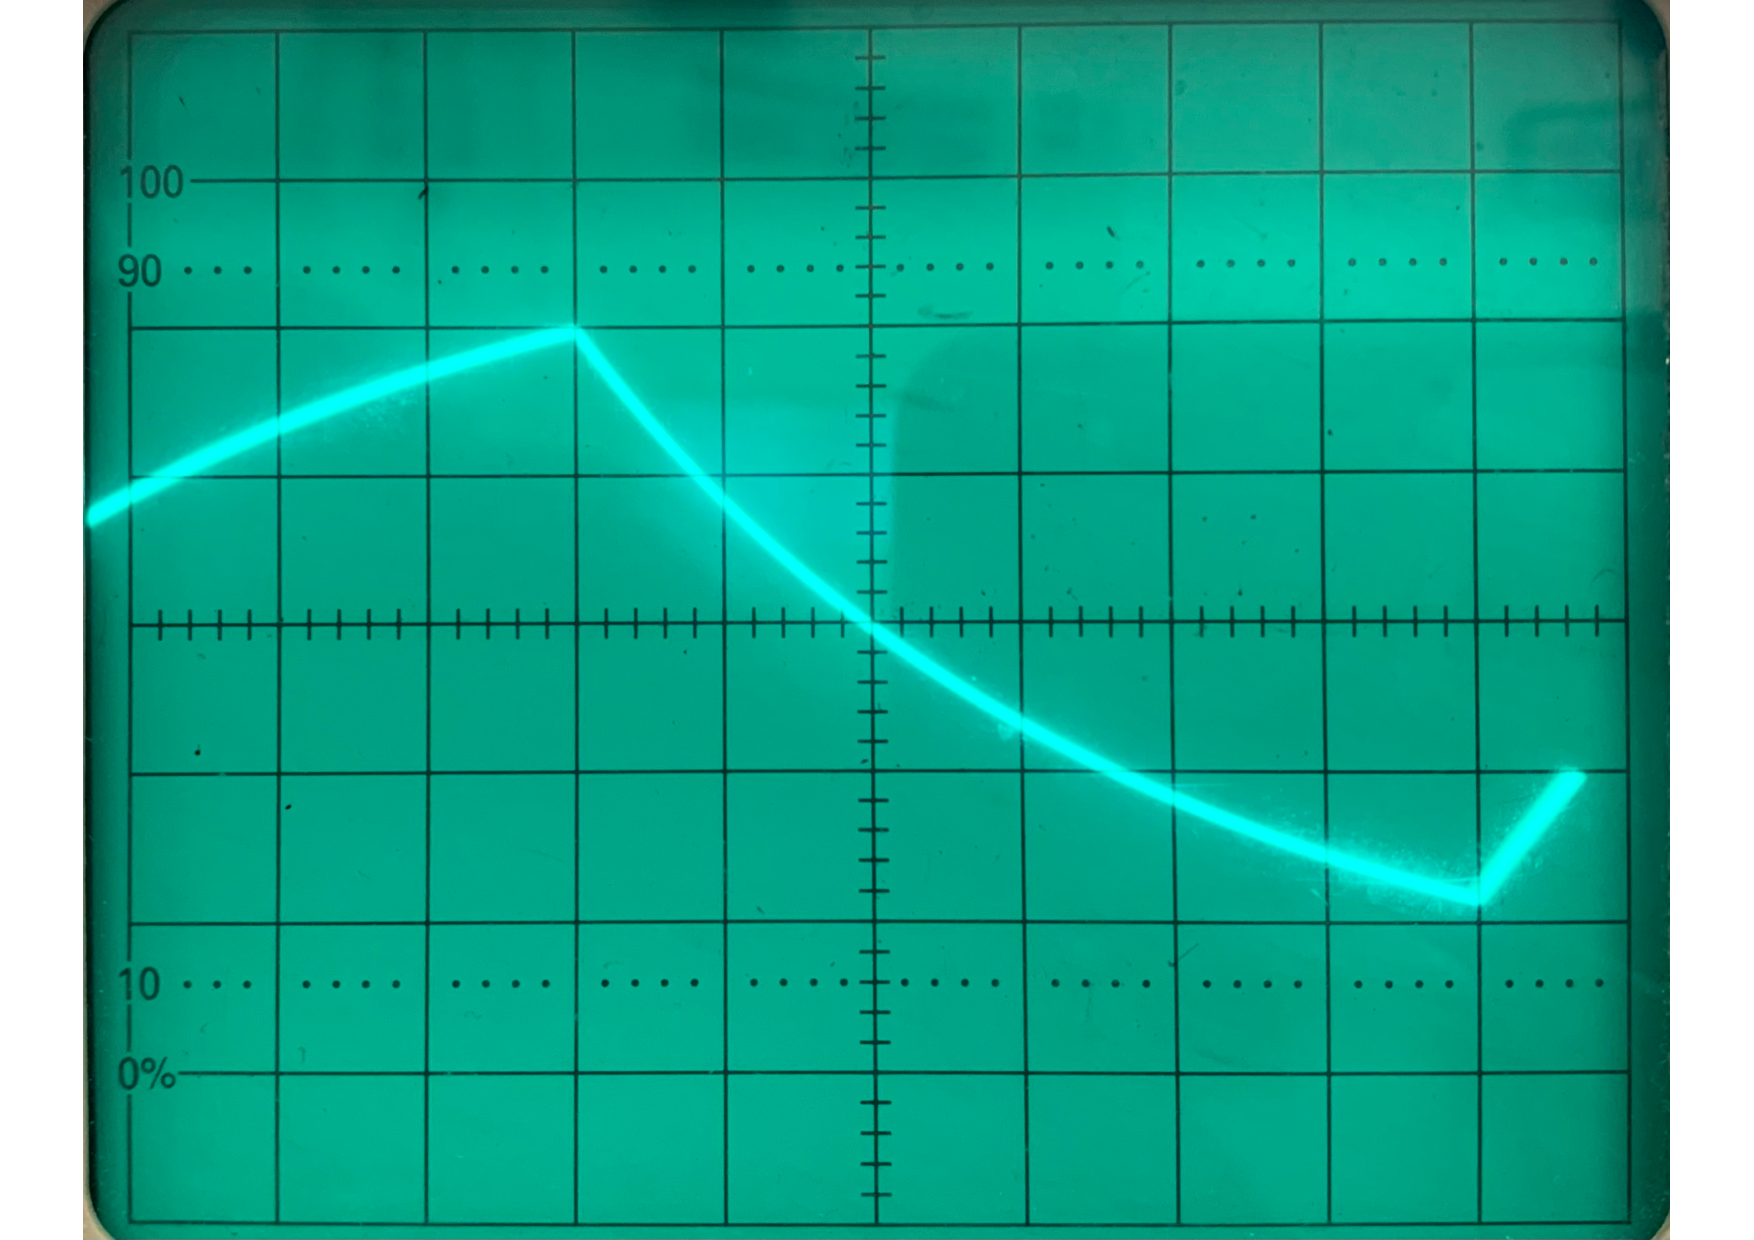
\includegraphics[height=10cm]{content/Aufgabe a - Rechteckspannung.pdf}
  \caption{Entladekurve des Kondensators mit Vorwiderstand}
  \label{fig:aufgabe a - rechteckspannung}
\end{figure}

\begin{figure}
  \begin{subfigure}{0.48\textwidth}
    \centering
    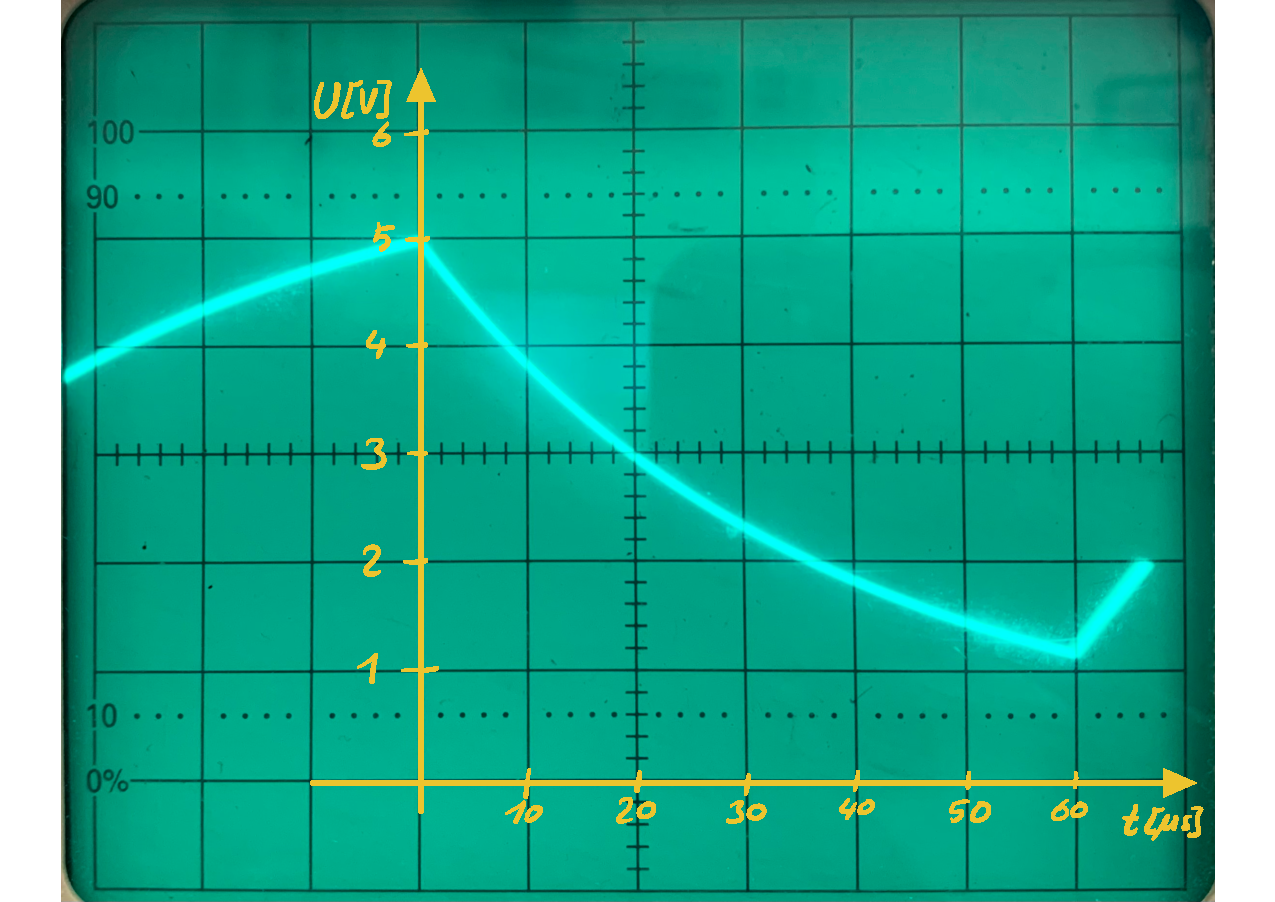
\includegraphics[height=5cm]{content/Aufgabe a - Gitter.pdf}
    \caption{Entladekurve mit Koordinatensystem}
    \label{fig:aufgabe a - gitter}
  \end{subfigure}
  \hfill
  \begin{subfigure}{0.48\textwidth}
    \centering
    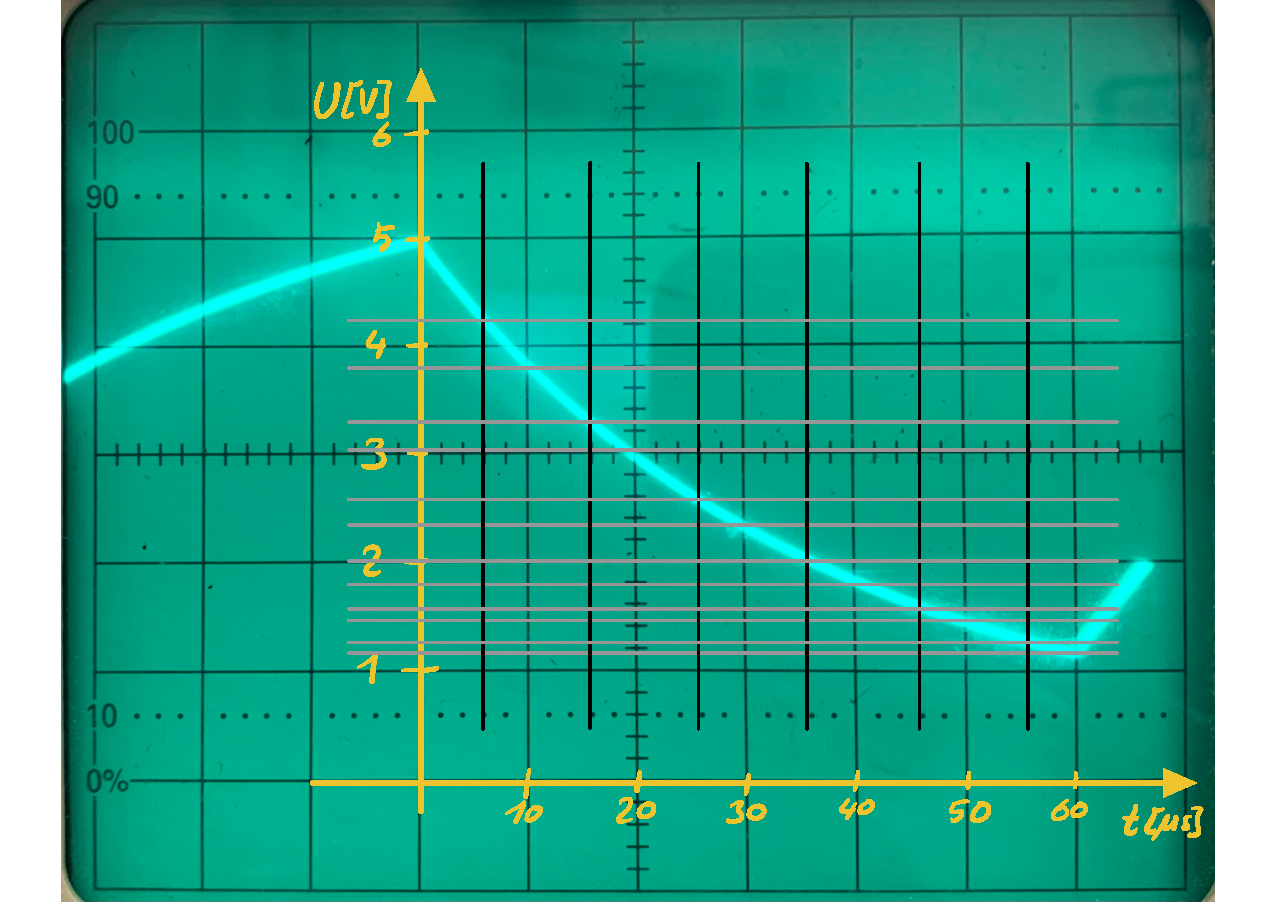
\includegraphics[height=5cm]{content/Aufgabe a - Hilfslinien.pdf}
    \caption{Entladekurve mit Hilfslinien}
    \label{fig:aufgabe a - hilfslinien}
  \end{subfigure}
  \caption{Entladekurve mit eingezeichnetem Koordinatensystem und Hilfslinien. Die %
    Skalierung wurde vorher durch Messung der Spannung der Rechteckspannung ermittelt.}
  \label{fig:aufgabe a - gitter und hilfslinien}
\end{figure}

\begin{table}
  \centering
  \caption{Darstellung der Messwertpaare, welche aus \autoref{fig:aufgabe a - gitter und hilfslinien} abgelesen wurden.}
  \label{tab:aufgabe a}
  \begin{tabular}{S[table-format=2.0] S[table-format=1.1]}
    \toprule
    {$f$ [Hz]} & {$U$ [V]} \\
    \midrule
    0 &  5,0 \\
    6	&  4,2 \\
    10 & 3,8 \\
    16 & 3,3 \\
    20 & 3,0 \\
    26 & 2,6 \\
    30 & 2,3 \\
    36 & 2,0 \\
    40 & 1,8 \\
    46 & 1,6 \\
    50 & 1,4 \\
    56 & 1,2 \\
    60 & 1,1 \\
    \bottomrule
  \end{tabular}
\end{table}

% ToDo:
% Lin Regr der Messwerte erstellen --> Plot
% RC bestimmen
% Fehlerrechnung

\subsection{Bestimmung der Zeitkonstante $RC$ über die Frequenabhängigkeit der Amplitude}
Die Spannung am Kondensator $A$ wird ebenso wie die Spannung der Sinusspannungsquelle $U_{0}$ bei variabler
Frequenz $f$ gemessen und tabellarisch in \autoref{tab:aufgabe c} dargestellt. Da sich bei der Messung $U_{0}$
als frequenzunabhängig und zu $U_{0} = 5,2$V bestimmen ließ (TEMPUS?!?!?!?!?!?!?!), ist dieser Wert aus Gründen der
Übersichtlichkeit nicht in der Tabelle aufgeführt. Das Teilungsverhältnis aus $\frac{A}{U_{0}}$ wird berechnet und
gleichermaßen dokumentiert. 

Die Wertepaare \{$f \symup{[Hz]}, \frac{A}{U_{0}}$\} aus \autoref{tab:aufgabe c} werden in ein Diagramm aufgetragen
und es wird eine nicht-lineare Ausgleichsrechnung mit den Python-Erweiterungen "numpy" \cite{numpy} und 
"matplotlib" \cite{matplotlib} (ÜBERPRÜFEN WELECHE BENUTZT!!!!!!!) durchgeführt. Die Fehlerrechnung für den Plot wird mit
der Python-Erweiterung \dq uncertainties" \cite{uncertainties} durchgeführt. Für den Plot werden nicht die
gerundeten Werte aus \autoref{tab:aufgabe c} verwendet, sondern die exakteren Werte $\frac{A}{U_{0}}$.
(IST DAS VERSTÄDLICH?!?!?!?!)

\begin{table}
  \centering
  \caption{Darstellung der Messwerte zu den Aufgabenteilen b) und c)}
  \label{tab:aufgabe c}
  \begin{tabular}{S[table-format=6.0] S[table-format=1.2] S[table-format=1.3]}
    \toprule
    {$f$ [Hz]} & {$A$ [V]} & {$\frac{A}{U_{0}}$} \\
    \midrule
    50     & 2,8	& 0.538 \\
    100    & 2,65 & 0.509 \\
    150    & 2,6  & 0.500 \\
    200    & 2,6  & 0.500 \\
    500    & 2,6  & 0.500 \\
    1000   & 2,5  & 0.480 \\
    1500   & 2,3  & 0.442 \\
    2000   & 2,05 & 0.394 \\
    3000   & 1,8  & 0.346 \\
    4000   & 1,5  & 0.288 \\
    5000   & 1,1  & 0.211 \\
    10000  & 0,68 & 0.130 \\
    20000  & 0,3  & 0.057 \\
    30000  & 0,22 & 0.042 \\
    50000  & 0,14 & 0.026 \\
    100000 & 0,07 & 0.013 \\
    \bottomrule
  \end{tabular}
\end{table}

\begin{table}
  \centering
  \caption{Darstellung der Messwerte zu den Aufgabenteilen b) und c)}
  \label{tab:aufgabe d}
  \begin{tabular}{S[table-format=6.0] S[table-format=3.1] S[table-format=5.0] S[table-format=1.3] S[table-format=1.3]}
    \toprule
    {$f$ [Hz]} & {$a$ [$\symup{\mu}$s]} & {$b$ [$\symup{\mu}$s]} & {$\varphi$ [rad]} & {$\varphi$ [$\frac{\pi}{\symup{rad}}$]}\\
    \midrule
    50      & 0	  & 20000 & 0.000 & 0.000 \\
    100     & 100 & 10000 & 0.062 & 0.020 \\
    150     &	100 & 6500  & 0.096 & 0.030 \\
    200     &	100 & 5000  & 0.125 & 0.040 \\ 
    500     &	100	& 2000  & 0.314 & 0.100 \\
    1000    &	100 & 1000  & 0.628 & 0.200 \\
    1500    & 55  & 630   & 0.548 & 0.174 \\
    2000    &	50  & 500   & 0.628 & 0.200 \\
    3000    & 44  & 330   & 0.837 & 0.266 \\
    4000    & 40  & 250   & 1.005 & 0.320 \\
    5000    & 36  & 200   & 1.131 & 0.360 \\
    10000   & 22  & 100   & 1.382 & 0.440 \\
    20000   & 12  & 52    & 1.450 & 0.461 \\
    30000   & 8   & 34    & 1.478 & 0.470 \\
    50000   & 4,9 & 20    & 1.539 & 0.490 \\
    100000  &	2,5 & 10    & 1.571 & 0.500 \\
    \bottomrule
  \end{tabular}
\end{table}

\begin{figure}
  \centering
  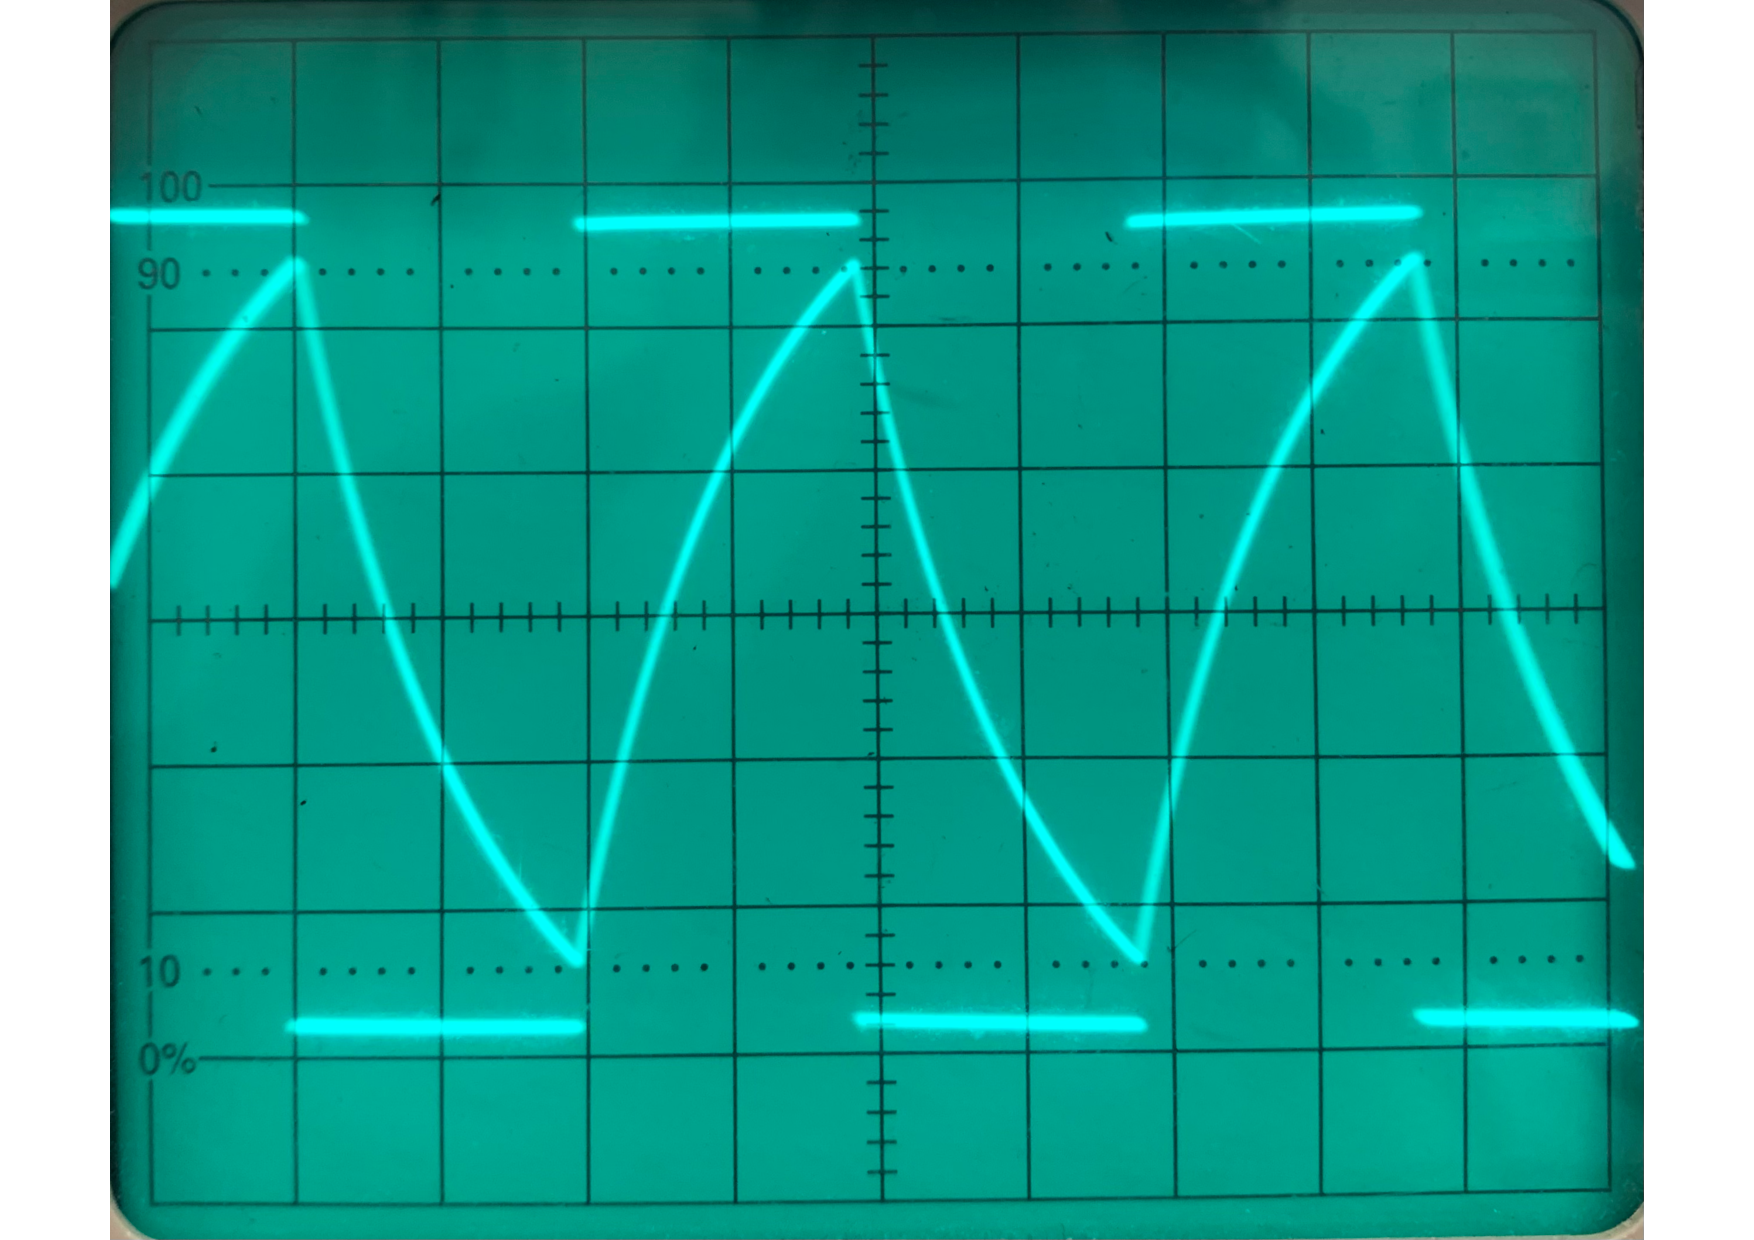
\includegraphics[height=10cm]{content/Aufgabe d - Rechteckspannung.pdf}
  \caption{Rechteckspannung $U_{0}$ und Kondensatorspannung mit $f=5$kHz}
  \label{fig:aufgabe d - rechteckspannung}
\end{figure}

\begin{figure}
  \centering
  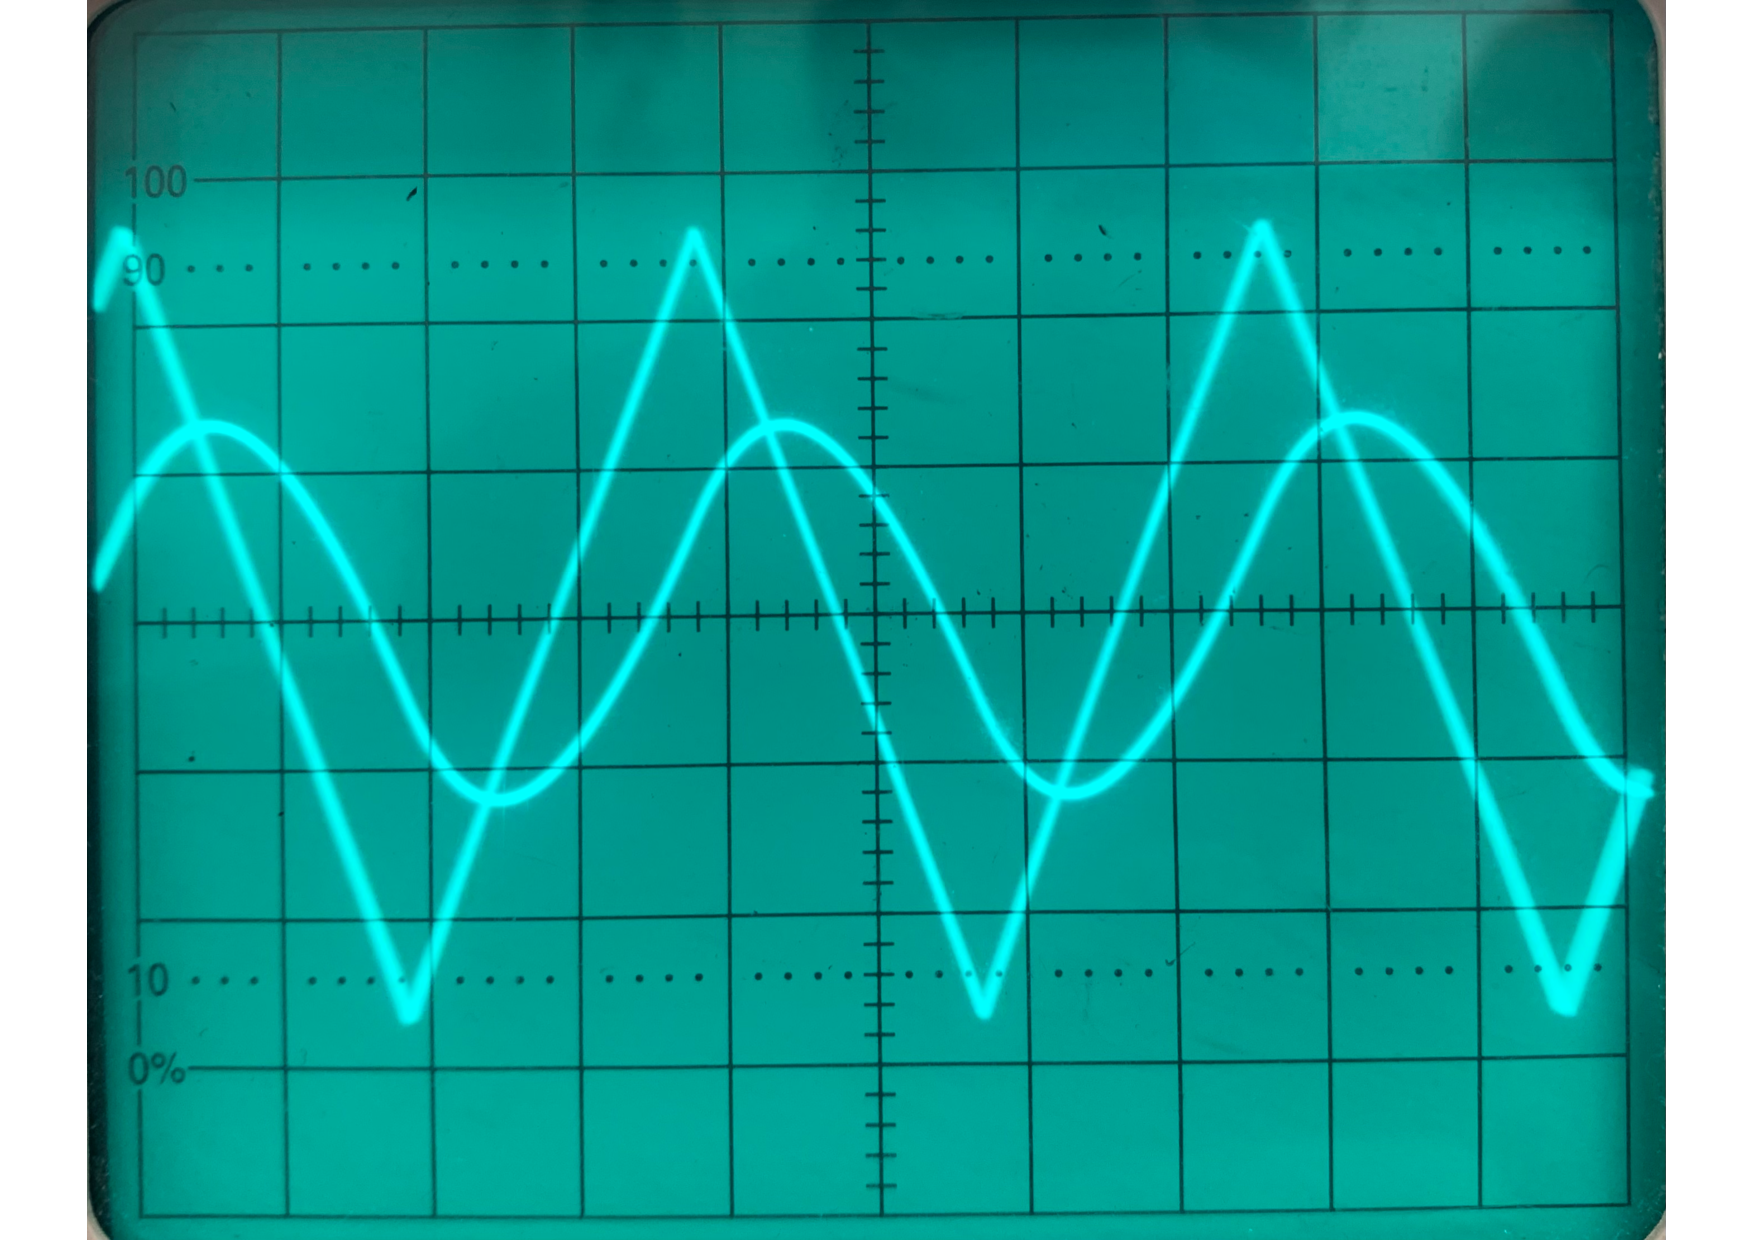
\includegraphics[height=10cm]{content/Aufgabe d - Dreieckspannung.pdf}
  \caption{Dreieckspannung $U_{0}$ und Kondensatorspannung mit $f=5$kHz}
  \label{fig:aufgabe d - dreieckspannung}
\end{figure}

\begin{figure}
  \centering
  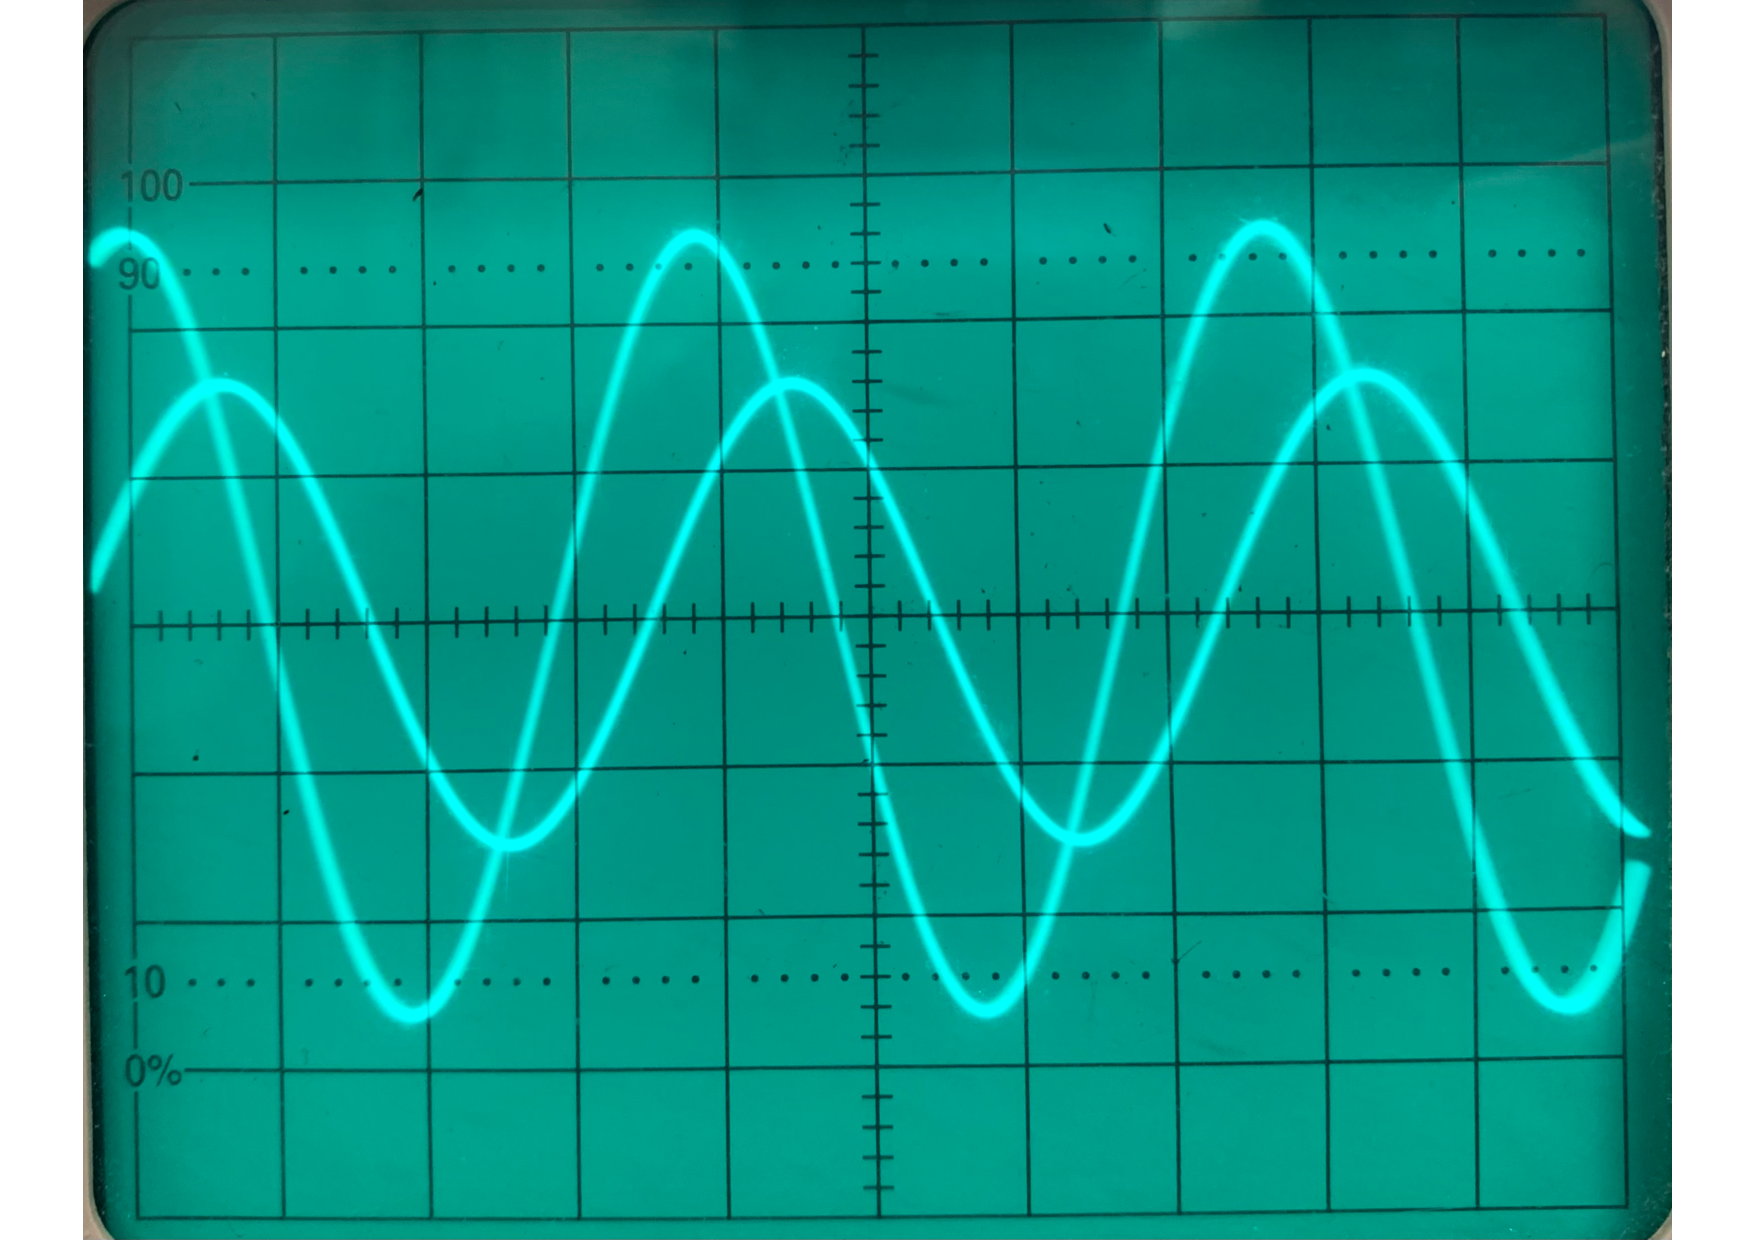
\includegraphics[height=10cm]{content/Aufgabe d - Sinusspannung.pdf}
  \caption{Sinusspannung $U_{0}$ und Kondensatorspannung mit $f=5$kHz}
  \label{fig:aufgabe d - sinusspannung}
\end{figure}
